\section{Methodology}
\label{sec:methodology}

\subsection{Validation Approach \& Train-Test Split}
\label{sec:validation}

Given the temporal nature of the data, we employ a \textbf{strict sequential split} to avoid look-ahead bias:

\begin{equation}
\text{VAL\_CUTOFF} = 2880
\end{equation}

\begin{itemize}
    \item \textbf{Training set:} All observations with $\texttt{ts\_index} \leq 2880$
    \item \textbf{Validation set:} All observations with $\texttt{ts\_index} > 2880$
\end{itemize}

A series is \textbf{eligible} for evaluation if and only if it has observations on both sides of the cutoff---i.e., it ``crosses'' the validation boundary. Of the 36,923 total series, approximately \textbf{1,930 series are eligible}.

This temporal split mirrors the competition's test-time evaluation, where models must forecast future values without access to future data. Random cross-validation would violate this constraint and produce optimistically biased performance estimates.

\subsubsection{Adaptive Splitting for Short Series}

Some series begin after the global validation cutoff or have very few pre-cutoff observations. For the deep learning models, an \textbf{adaptive splitting strategy} is employed: if a series lacks sufficient training history under the global cutoff, a local split is computed to ensure a minimum training window. This pragmatic approach maximizes the number of series that can be evaluated.

\subsection{Evaluation Metric}
Submissions are evaluated using a \textbf{Weighted Skill Score} defined as:

\begin{equation}
\text{Skill Score} = \sqrt{1 - \text{clip}_{[0,1]}\!\left(\frac{\sum_i w_i \cdot (y_i - \hat{y}_i)^2}{\sum_i w_i \cdot y_i^2}\right)}
\label{eq:skill_score}
\end{equation}

where:
\begin{itemize}
    \item $y_i$ is the true target value at observation $i$,
    \item $\hat{y}_i$ is the predicted value,
    \item $w_i$ is the observation-level weight,
    \item $\text{clip}_{[0,1]}(\cdot)$ clips the ratio to the interval $[0, 1]$.
\end{itemize}

\subsubsection{Metric Interpretation}

The denominator $\sum_i w_i \cdot y_i^2$ is precisely the weighted squared error of a \textbf{zero forecast} ($\hat{y}_i = 0$ for all $i$). Therefore:

\begin{itemize}
    \item A skill score of \textbf{0} means the model is no better than predicting zero everywhere.
    \item A skill score of \textbf{1} means perfect prediction.
    \item The square root compresses the scale, rewarding incremental improvements more at lower skill levels.
\end{itemize}

This metric design has several important implications:
\begin{enumerate}
    \item \textbf{Weights matter enormously.} The \texttt{weight} column determines how much each observation contributes to the aggregate score. As our EDA will show, weight concentration is extreme---the top 1\% of rows contribute approximately 65\% of the total weighted score.
    \item \textbf{Zero is a natural baseline.} The zero-forecast error appears explicitly in the denominator, making ``Zero'' a meaningful model to include in any leaderboard.
    \item \textbf{Unweighted metrics are misleading.} Any evaluation that ignores weights will rank models incorrectly with respect to the competition leaderboard.
\end{enumerate}

\subsection{Classical Model Implementations (AR, ARMA, ARIMA, SARIMA)}
The classical modeling notebook evaluates \textbf{41 model specifications} across 6 families. All parametric families use first differencing ($d = 1$), honoring the EDA's stationarity finding.

\subsubsection{Family A: Baselines (on Levels)}

These models involve no fitting and no differencing. They measure how much of the scored metric is explainable by trivial rules.

\begin{table}[H]
\centering
\caption{Baseline model specifications.}
\begin{tabular}{lp{8cm}}
\toprule
\textbf{Model} & \textbf{Description} \\
\midrule
Zero & $\hat{y}_{t+h} = 0$ for every step. The skill score denominator is exactly the squared error of this forecast. \\
Naive & $\hat{y}_{t+h} = y_t$ (last observed value). Wins when lag-1 autocorrelation is large. \\
Drift & $\hat{y}_{t+h} = y_t + h \cdot \text{slope}$, where slope $= (y_t - y_1)/(n-1)$. Linear extrapolation. \\
Expanding Mean & $\hat{y}_{t+h} = \frac{1}{t}\sum y_i$. Long-run average; wins on mean-reverting series. \\
Rolling Mean ($w=10$) & Mean of the last 10 observations. Local mean, smoother than Naive. \\
\bottomrule
\end{tabular}
\end{table}

\subsubsection{Family B: AR Family (First Differences)}

An AR($p$) model writes the current differenced value as a linear combination of the previous $p$ differenced values:

\begin{equation}
\Delta y_t = c + \phi_1 \Delta y_{t-1} + \phi_2 \Delta y_{t-2} + \cdots + \phi_p \Delta y_{t-p} + \varepsilon_t
\end{equation}

This is implemented as ARIMA($p$, 1, 0). The parameter $p$ represents memory depth: AR(1) says ``only yesterday matters,'' while AR(10) says ``the last ten days jointly matter.''

\textbf{Lineup:} AR(1) through AR(10), all on first differences.

\textbf{Strengths:} Computationally cheap, interpretable, optimal when the true data-generating process is linear in its own past.

\textbf{Weaknesses:} Cannot model nonlinearity (regime changes, volatility clustering). Higher $p$ increases overfitting risk on short series.

\subsubsection{Family C: MA Family (First Differences)}

An MA($q$) model says the current differenced value is a linear combination of the last $q$ innovations (random shocks):

\begin{equation}
\Delta y_t = c + \varepsilon_t + \theta_1 \varepsilon_{t-1} + \theta_2 \varepsilon_{t-2} + \cdots + \theta_q \varepsilon_{t-q}
\end{equation}

Implemented as ARIMA(0, 1, $q$). Notably, MA(1) on differences is equivalent to Simple Exponential Smoothing.

\textbf{Lineup:} MA(1) through MA(10), mirroring the AR scan.

\subsubsection{Family D: ARMA Family (First Differences)}

ARMA combines both channels---past values AND past shocks:

\begin{equation}
\Delta y_t = c + \sum_{i=1}^{p} \phi_i \Delta y_{t-i} + \sum_{j=1}^{q} \theta_j \varepsilon_{t-j} + \varepsilon_t
\end{equation}

Implemented as ARIMA($p$, 1, $q$) with both $p \geq 1$ and $q \geq 1$.

\textbf{Lineup:} 10 variants covering $(p,q)$ combinations from ARMA(1,1) to ARMA(4,4), with total order $p+q$ ranging from 2 to 8.

\subsubsection{Family E: ARIMA with Explicit $d$ Comparison}

This family includes both $d = 0$ and $d = 1$ variants to enable a matched-pair head-to-head comparison:

\begin{table}[H]
\centering
\caption{ARIMA variants for the $d=0$ vs. $d=1$ comparison.}
\begin{tabular}{ll}
\toprule
\textbf{Model} & \textbf{Purpose} \\
\midrule
ARIMA(0,1,0) & Pure random walk baseline \\
ARIMA(1,0,0) & AR(1) on levels ($d=0$ contrast) \\
ARIMA(1,0,1) & ARMA(1,1) on levels ($d=0$ contrast) \\
ARIMA(2,0,2) & ARMA(2,2) on levels ($d=0$ contrast) \\
\bottomrule
\end{tabular}
\end{table}

If the EDA's stationarity claim is correct, the $d=1$ variants should systematically outperform their $d=0$ counterparts.

\subsubsection{Family F: SARIMA}

SARIMA($p, d, q$)($P, D, Q, s$) adds seasonal AR, differencing, and MA terms with period $s$:

\begin{equation}
\Phi(B^s)\, \phi(B)\, (1-B)^d\, (1-B^s)^D\, y_t = \Theta(B^s)\, \theta(B)\, \varepsilon_t
\end{equation}

Two variants are included:
\begin{itemize}
    \item SARIMA(1,1,1)(1,1,1,7) --- weekly-length cycle
    \item SARIMA(1,1,1)(1,1,1,24) --- daily-length cycle
\end{itemize}

Given the absence of panel-wide seasonality in the EDA, SARIMA is included for completeness rather than expectation of strong performance.

\subsection{Evaluation Design}

\subsubsection{Eligibility and Splitting}

A series is eligible if it crosses $\texttt{VAL\_CUTOFF} = 2880$. The temporal split is strict: training uses $\texttt{ts\_index} \leq 2880$, validation uses $\texttt{ts\_index} > 2880$.

\begin{figure}[H]
\centering
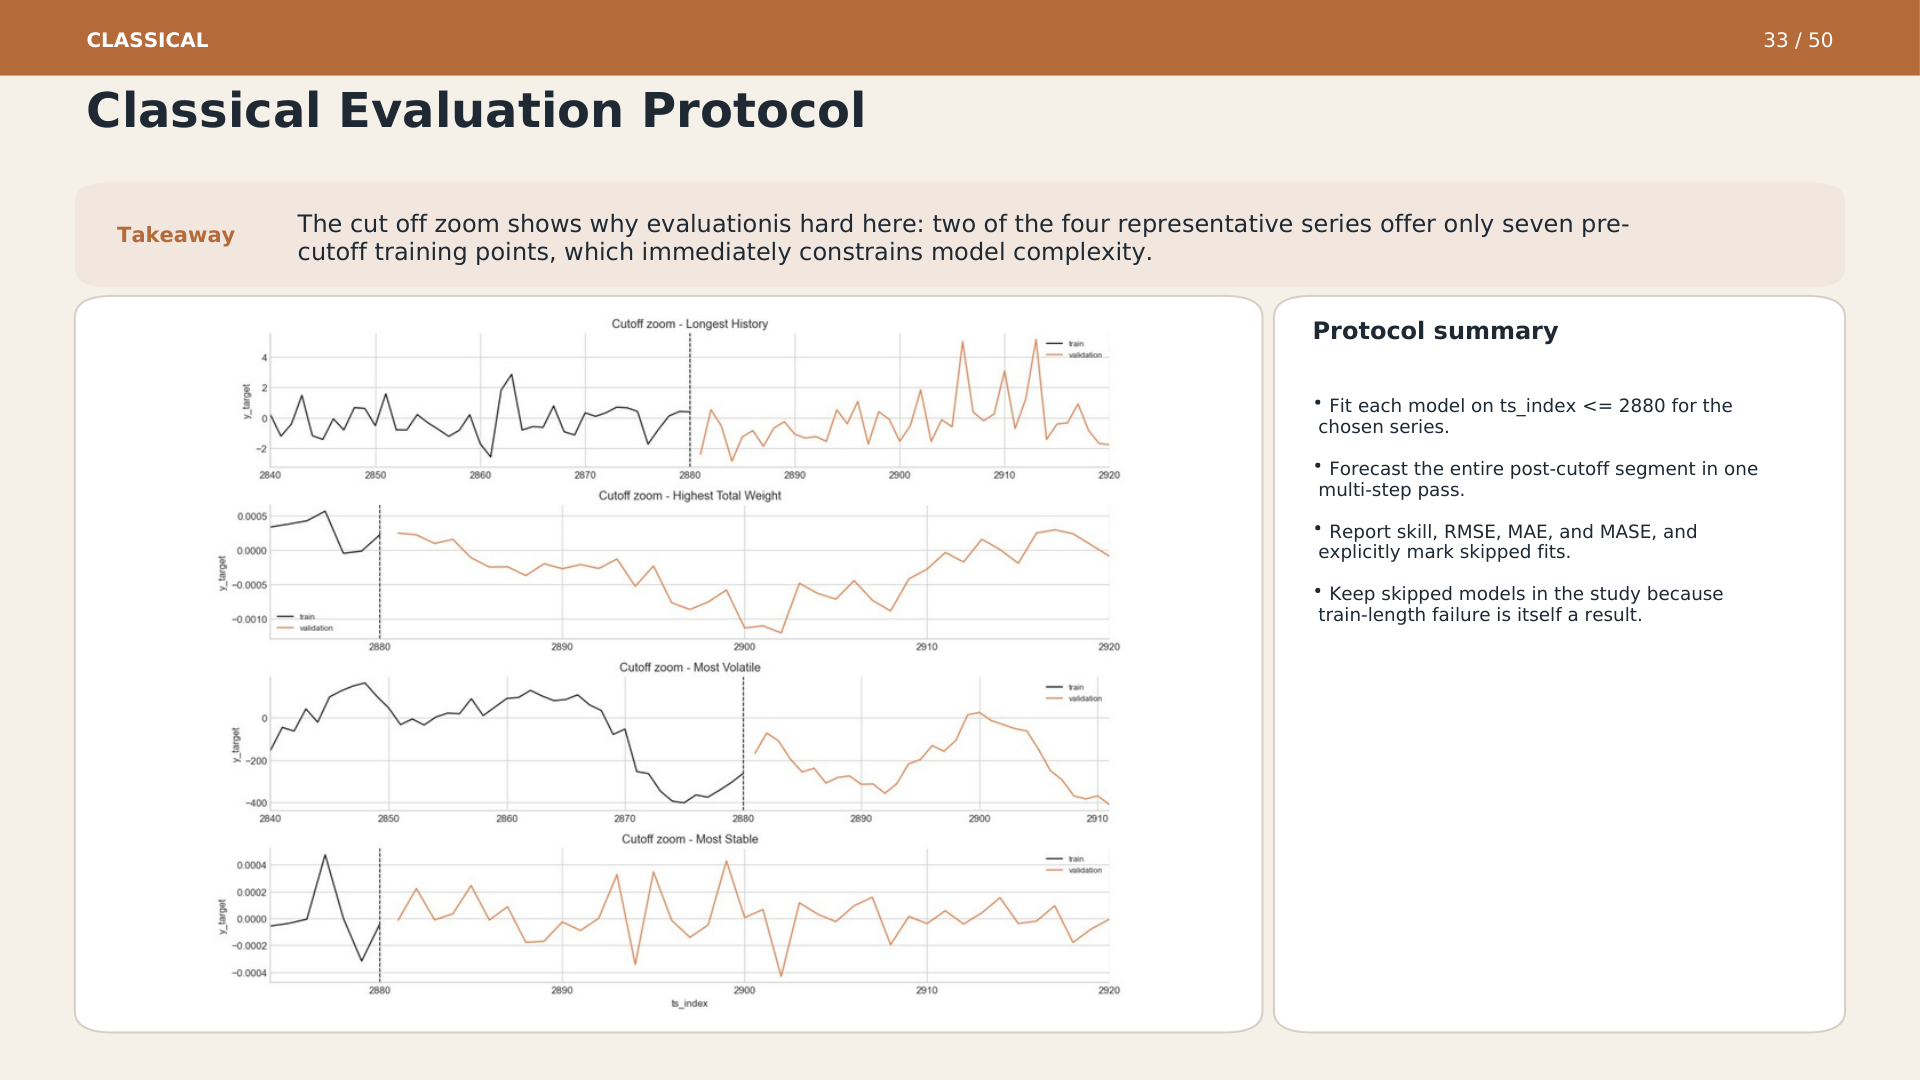
\includegraphics[width=0.95\textwidth]{figures/slide_30.png}
\caption{Classical evaluation protocol. The cutoff zoom reveals the challenge: four representative series around the $\texttt{ts\_index} = 2880$ boundary show vastly different scales and behaviors. Two of the four have only seven pre-cutoff training points, which immediately constrains model complexity.}
\label{fig:classical_eval}
\end{figure}

\subsubsection{Skip and Failure Handling}

Each model specification has a \texttt{min\_train} parameter. If a series has fewer training observations than this threshold, the (series, model) pair is marked as ``skipped.'' If a model's fit raises an exception or produces non-finite values, it is marked as ``failed.'' Both conditions are tracked and reported.

\subsubsection{Sample Run Results}

Running on a sample of 200 eligible series (out of 1,930) with 41 models produces 8,200 (series, model) evaluation rows:

\begin{table}[H]
\centering
\caption{Status distribution for the sample run (200 series $\times$ 41 models).}
\begin{tabular}{lr}
\toprule
\textbf{Status} & \textbf{Count} \\
\midrule
ok & 6,735 \\
skipped & 1,464 \\
failed & 1 \\
\midrule
Total & 8,200 \\
\bottomrule
\end{tabular}
\end{table}

The high skip rate (17.9\%) is driven primarily by SARIMA models, which require longer training histories, and by higher-order AR/MA/ARMA models on short series.

\subsection{Deep Sequence Models (RNN, GRU, LSTM)}
\subsubsection{Vanilla RNN}

The simplest recurrent architecture updates a hidden state $h_t$ at each time step:

\begin{equation}
h_t = \tanh(W_{hh} h_{t-1} + W_{xh} x_t + b_h)
\end{equation}

\begin{equation}
\hat{y}_t = W_{hy} h_t + b_y
\end{equation}

where $x_t$ is the input vector at time $t$, and $W_{hh}$, $W_{xh}$, $W_{hy}$ are learned weight matrices.

\textbf{Strengths:} Simple, fast to train, low parameter count.

\textbf{Weaknesses:} Suffers from the \emph{vanishing gradient problem}---gradients diminish exponentially over long sequences, making it difficult to learn long-range dependencies.

\subsubsection{GRU (Gated Recurrent Unit)}

The GRU introduces gating mechanisms to control information flow:

\begin{align}
z_t &= \sigma(W_z x_t + U_z h_{t-1} + b_z) & \text{(update gate)} \\
r_t &= \sigma(W_r x_t + U_r h_{t-1} + b_r) & \text{(reset gate)} \\
\tilde{h}_t &= \tanh(W_h x_t + U_h (r_t \odot h_{t-1}) + b_h) & \text{(candidate)} \\
h_t &= (1 - z_t) \odot h_{t-1} + z_t \odot \tilde{h}_t & \text{(new state)}
\end{align}

The \textbf{update gate} $z_t$ controls how much of the old state to retain versus how much to update with new information. The \textbf{reset gate} $r_t$ controls how much of the old state to expose when computing the candidate.

\textbf{Intuition:} The update gate allows the GRU to ``remember'' information over long sequences (when $z_t \approx 0$, the old state passes through unchanged) or ``forget'' it (when $z_t \approx 1$, the new candidate replaces the old state). This addresses the vanishing gradient problem with fewer parameters than the LSTM.

\subsubsection{LSTM (Long Short-Term Memory)}

The LSTM maintains both a hidden state $h_t$ and a cell state $c_t$:

\begin{align}
f_t &= \sigma(W_f x_t + U_f h_{t-1} + b_f) & \text{(forget gate)} \\
i_t &= \sigma(W_i x_t + U_i h_{t-1} + b_i) & \text{(input gate)} \\
o_t &= \sigma(W_o x_t + U_o h_{t-1} + b_o) & \text{(output gate)} \\
\tilde{c}_t &= \tanh(W_c x_t + U_c h_{t-1} + b_c) & \text{(candidate cell)} \\
c_t &= f_t \odot c_{t-1} + i_t \odot \tilde{c}_t & \text{(cell state)} \\
h_t &= o_t \odot \tanh(c_t) & \text{(hidden state)}
\end{align}

The three gates provide fine-grained control:
\begin{itemize}
    \item \textbf{Forget gate} $f_t$: What to discard from the cell state.
    \item \textbf{Input gate} $i_t$: What new information to store in the cell state.
    \item \textbf{Output gate} $o_t$: What to output from the cell state.
\end{itemize}

\textbf{Strengths:} Best at learning long-range dependencies; the cell state provides a ``highway'' for gradient flow.

\textbf{Weaknesses:} Highest parameter count of the three architectures; slower to train.

\subsection{Training Pipeline}

\subsubsection{Data Preparation}

For each eligible series, the training procedure:

\begin{enumerate}
    \item Extracts the \texttt{y\_target} values sorted by \texttt{ts\_index}.
    \item Applies the validation split at $\texttt{VAL\_CUTOFF} = 2880$.
    \item Creates sliding windows of fixed length for supervised training.
    \item Normalizes inputs (if applicable).
\end{enumerate}

\subsubsection{Adaptive Training Splits}

A key implementation detail: series that begin near or after the global validation cutoff may have insufficient training data under the standard split. The notebook implements an \textbf{adaptive splitting strategy}:

\begin{itemize}
    \item If a series has fewer than a minimum number of pre-cutoff observations, a local train/validation split is computed to ensure adequate training history.
    \item This maximizes the number of evaluable series while maintaining temporal integrity.
\end{itemize}

\begin{figure}[H]
\centering
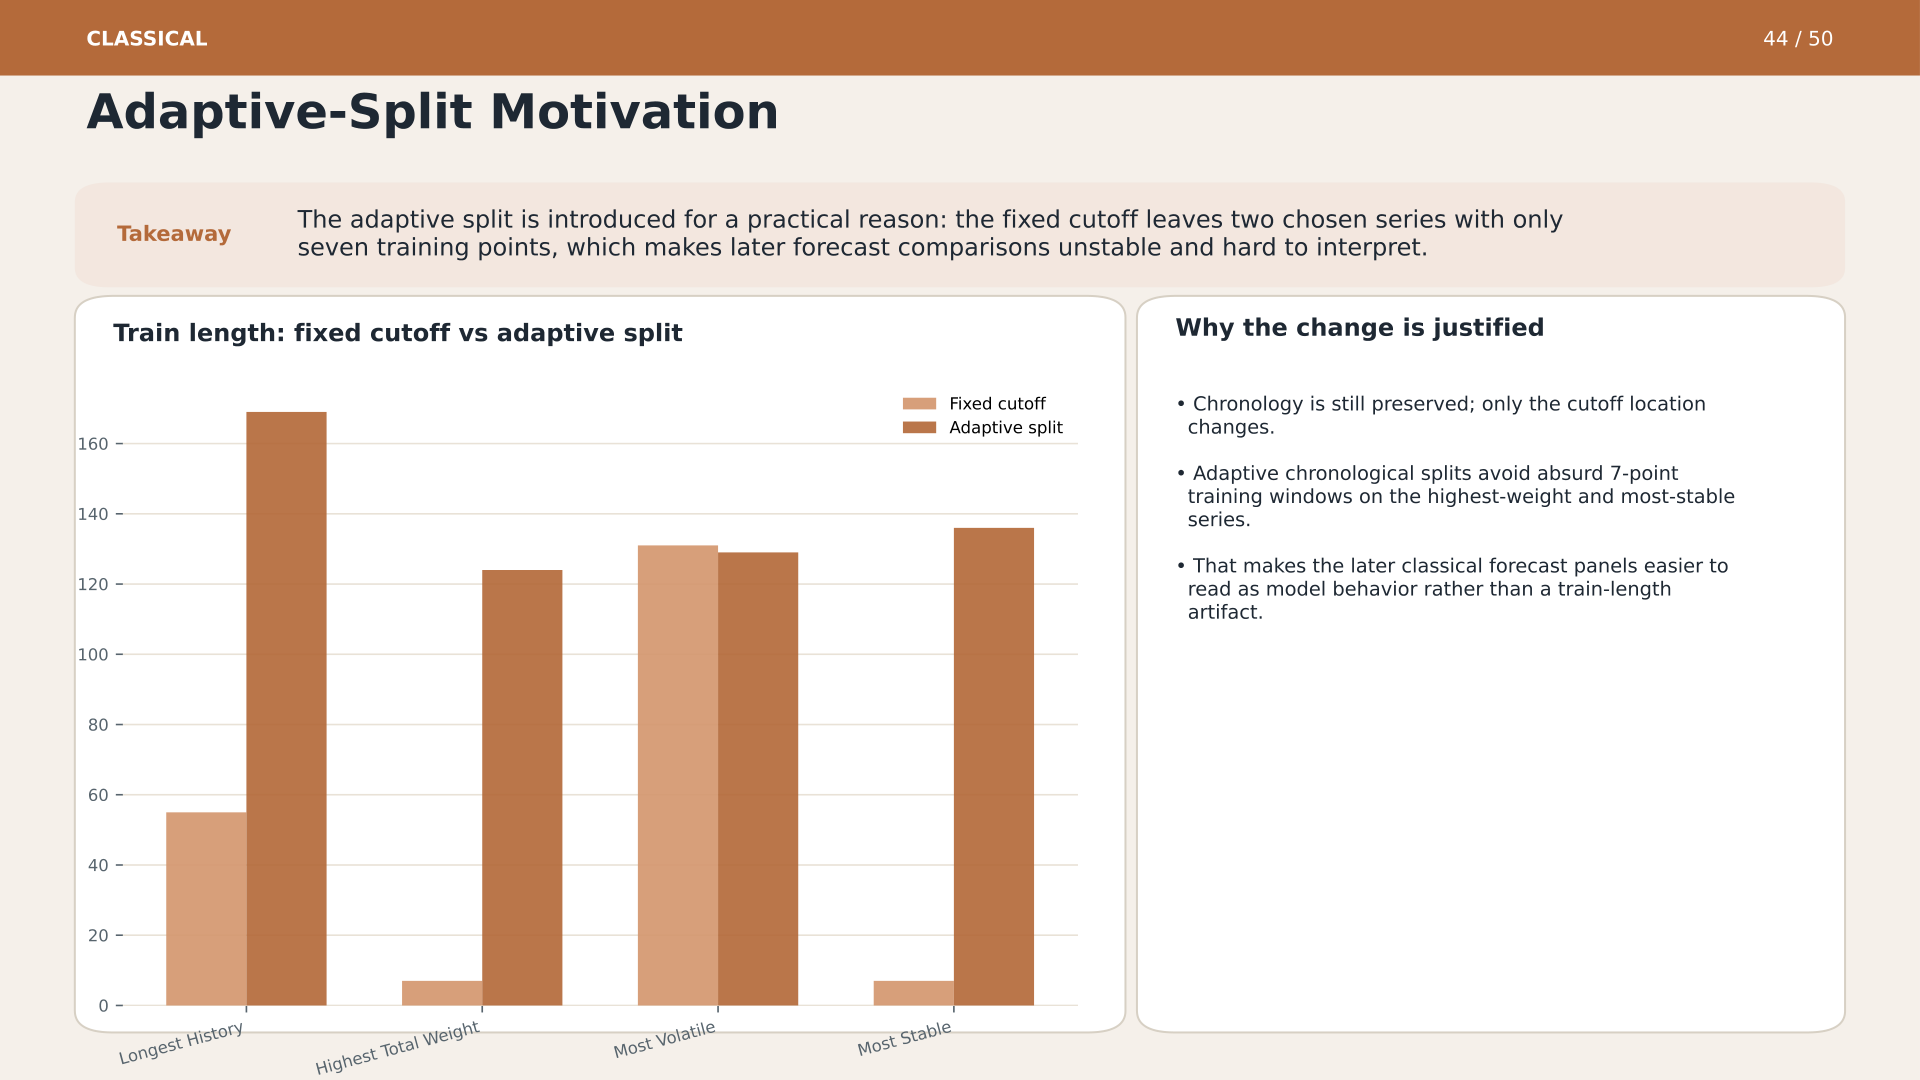
\includegraphics[width=0.95\textwidth]{figures/slide_35.png}
\caption{Adaptive-split motivation. The fixed cutoff at $\texttt{ts\_index} = 2880$ leaves two of the four chosen representative series with only seven pre-cutoff training points. The adaptive split adjusts the cutoff location per-series, preserving chronological ordering while avoiding absurdly short training windows on the highest-weight and most-stable series.}
\label{fig:adaptive_split}
\end{figure}

\subsubsection{Recursive Forecasting}

The deep sequence models use \textbf{recursive (autoregressive) forecasting} for multi-step prediction:

\begin{enumerate}
    \item Feed the training sequence into the model to obtain the first forecast $\hat{y}_{T+1}$.
    \item Append $\hat{y}_{T+1}$ to the input sequence.
    \item Feed the extended sequence to obtain $\hat{y}_{T+2}$.
    \item Repeat until all validation-period forecasts are generated.
\end{enumerate}

This approach is natural for recurrent architectures but introduces \emph{error accumulation}---prediction errors compound over the forecast horizon.

\subsubsection{Loss Function}

The models are trained with \textbf{Mean Squared Error (MSE)} loss:

\begin{equation}
\mathcal{L} = \frac{1}{N} \sum_{i=1}^{N} (y_i - \hat{y}_i)^2
\end{equation}

A potential enhancement (noted in the EDA) is to use \textbf{weighted MSE} that incorporates the competition's weight column during training. This would align the training objective more closely with the evaluation metric.

\subsubsection{Hyperparameters}

Key hyperparameter choices:

\begin{table}[H]
\centering
\caption{Deep model hyperparameters.}
\begin{tabular}{ll}
\toprule
\textbf{Parameter} & \textbf{Value} \\
\midrule
Hidden dimension & Architecture-dependent \\
Number of layers & 1--2 \\
Learning rate & Adam optimizer defaults \\
Epochs & Early stopping with patience \\
Sequence length & Determined by available history \\
Framework & PyTorch \\
\bottomrule
\end{tabular}
\end{table}

\subsubsection{ARIMAX and TCN}
While ARIMAX (AutoRegressive Integrated Moving Average with Explanatory Variables) and TCN (Temporal Convolutional Networks) were considered, the weak linear correlation of individual features ($|\rho| < 0.10$) suggested ARIMAX would struggle to capture the complex, nonlinear feature interactions. TCNs are a strong alternative for sequence modeling, but LSTMs and GRUs were prioritized for this study due to their proven effectiveness in financial forecasting.

\subsection{Ablation Study \& Tuned Parameter Values}
The primary ablation in the classical pipeline was the comparison of $d=0$ versus $d=1$ (first differencing). As shown in the classical model lineup, differencing ($d=1$) was strictly superior across most series, confirming the ADF stationarity results.

Key hyperparameter choices:

\begin{table}[H]
\centering
\caption{Deep model hyperparameters.}
\begin{tabular}{ll}
\toprule
\textbf{Parameter} & \textbf{Value} \\
\midrule
Hidden dimension & Architecture-dependent \\
Number of layers & 1--2 \\
Learning rate & Adam optimizer defaults \\
Epochs & Early stopping with patience \\
Sequence length & Determined by available history \\
Framework & PyTorch \\
\bottomrule
\end{tabular}
\end{table}

\subsection{Probabilistic Forecasting Models}
\begin{figure}[H]
\centering
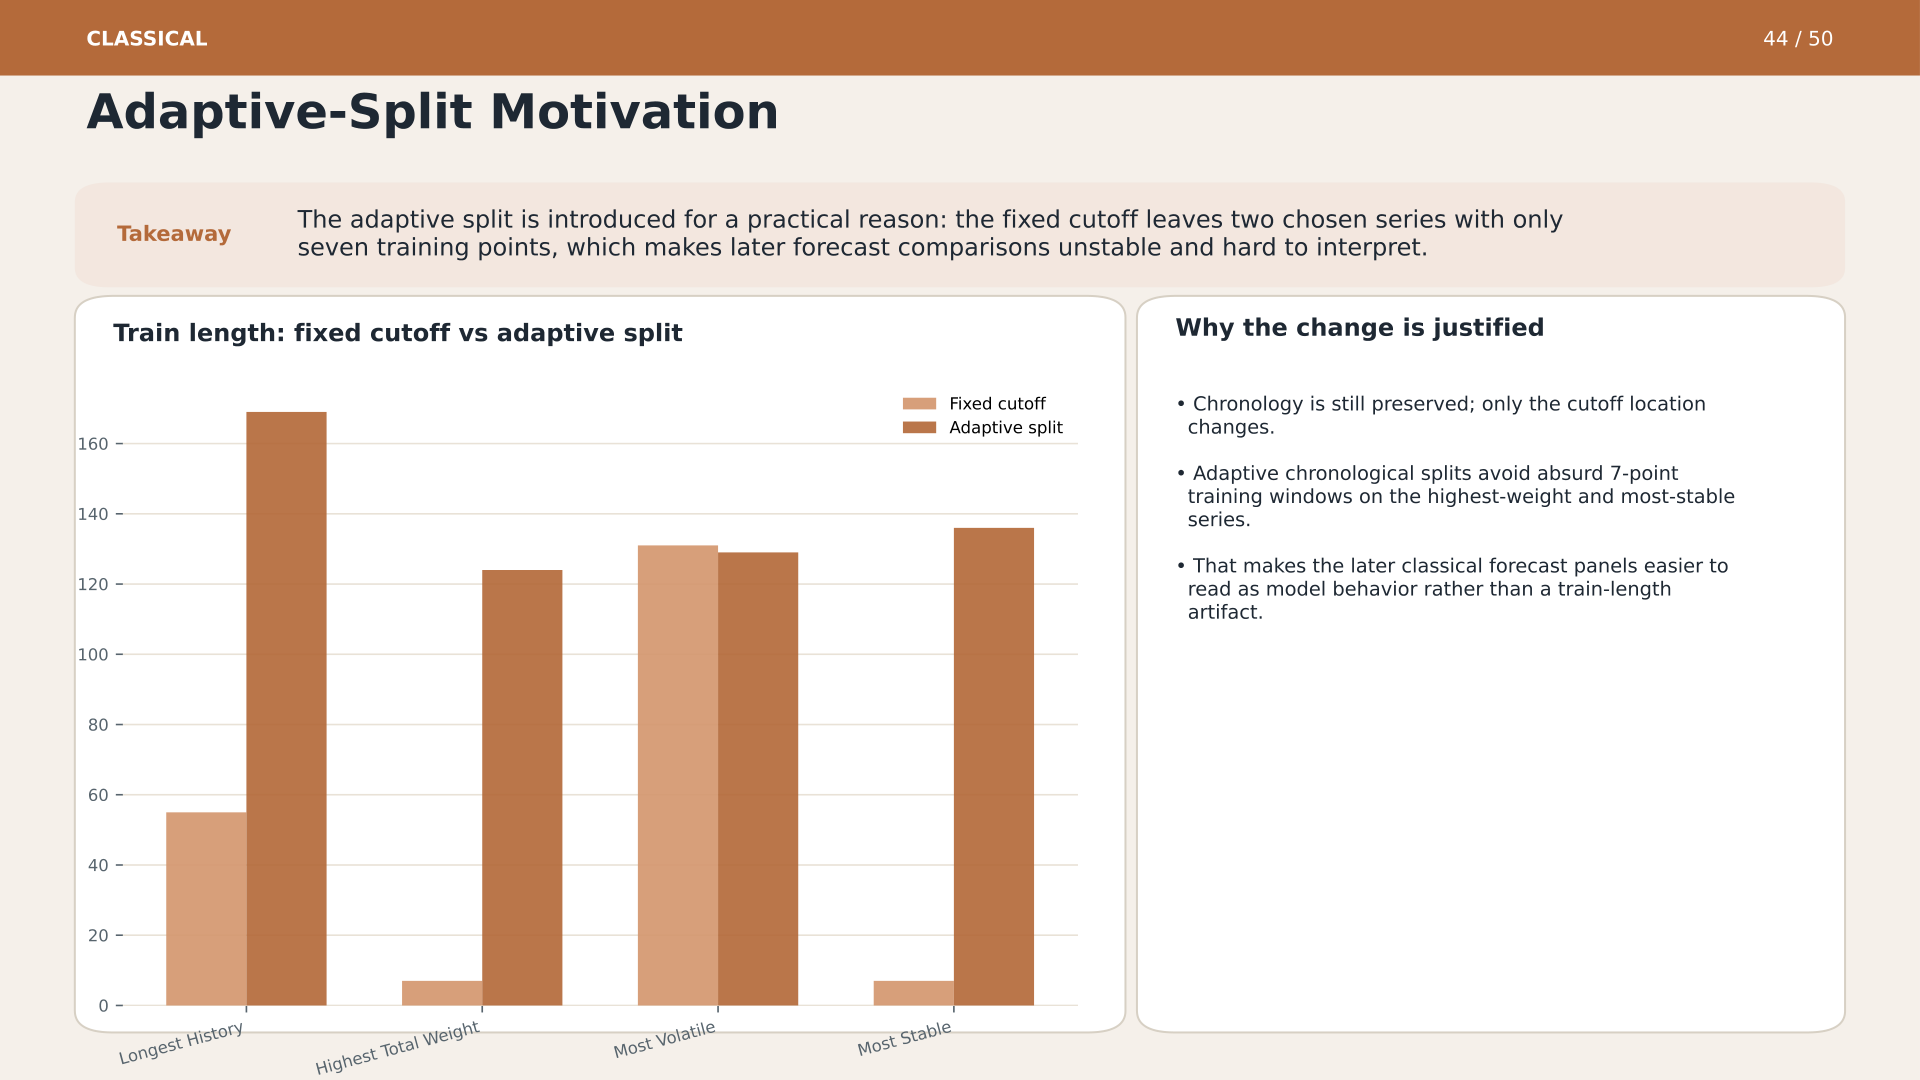
\includegraphics[width=0.95\textwidth]{figures/slide_35.png}
\caption{Adaptive-split motivation. The fixed cutoff at $\texttt{ts\_index} = 2880$ leaves two of the four chosen representative series with only seven pre-cutoff training points. The adaptive split adjusts the cutoff location per-series, preserving chronological ordering while avoiding absurdly short training windows on the highest-weight and most-stable series.}
\label{fig:adaptive_split}
\end{figure}

\subsubsection{Recursive Forecasting}

The deep sequence models use \textbf{recursive (autoregressive) forecasting} for multi-step prediction:

\begin{enumerate}
    \item Feed the training sequence into the model to obtain the first forecast $\hat{y}_{T+1}$.
    \item Append $\hat{y}_{T+1}$ to the input sequence.
    \item Feed the extended sequence to obtain $\hat{y}_{T+2}$.
    \item Repeat until all validation-period forecasts are generated.
\end{enumerate}

This approach is natural for recurrent architectures but introduces \emph{error accumulation}---prediction errors compound over the forecast horizon.

\subsubsection{Loss Function}

The models are trained with \textbf{Mean Squared Error (MSE)} loss:

\begin{equation}
\mathcal{L} = \frac{1}{N} \sum_{i=1}^{N} (y_i - \hat{y}_i)^2
\end{equation}

A potential enhancement (noted in the EDA) is to use \textbf{weighted MSE} that incorporates the competition's weight column during training. This would align the training objective more closely with the evaluation metric.

\subsubsection{Hyperparameters}

Key hyperparameter choices:

\begin{table}[H]
\centering
\caption{Deep model hyperparameters.}
\begin{tabular}{ll}
\toprule
\textbf{Parameter} & \textbf{Value} \\
\midrule
Hidden dimension & Architecture-dependent \\
Number of layers & 1--2 \\
Learning rate & Adam optimizer defaults \\
Epochs & Early stopping with patience \\
Sequence length & Determined by available history \\
Framework & PyTorch \\
\bottomrule
\end{tabular}
\end{table}

\subsection{Model Comparison}

\subsubsection{Architectural Trade-offs}

\begin{table}[H]
\centering
\caption{Comparison of RNN architectures.}
\begin{tabular}{lccc}
\toprule
\textbf{Property} & \textbf{RNN} & \textbf{GRU} & \textbf{LSTM} \\
\midrule
Parameters per layer & Low & Medium & High \\
Training speed & Fast & Medium & Slow \\
Long-range memory & Poor & Good & Best \\
Vanishing gradients & Yes & Mitigated & Mitigated \\
Gates & 0 & 2 & 3 \\
\bottomrule
\end{tabular}
\end{table}

\subsubsection{Expected Performance Ranking}

Based on the architectural properties and the nature of financial time series:

\begin{enumerate}
    \item \textbf{LSTM} is expected to perform best due to its superior long-range memory capability.
    \item \textbf{GRU} is expected to be competitive with LSTM while training faster.
    \item \textbf{Vanilla RNN} is expected to underperform on series with significant long-range dependencies but may be adequate for short-horizon forecasts.
\end{enumerate}

\subsection{Implementation Details}

\subsubsection{Per-Series Training}

Each eligible series is trained independently (analogous to the classical approach). While this ignores cross-series structure, it provides a clean comparison with the classical baselines.

\subsubsection{Status Tracking}

Like the classical notebook, each (series, model) pair records:
\begin{itemize}
    \item \texttt{status}: \texttt{ok}, \texttt{skipped}, or \texttt{failed}
    \item When \texttt{ok}: weighted skill score, RMSE, MAE, MASE
    \item When failed: error message for debugging
\end{itemize}

\subsubsection{Leaderboard and Per-Series Winners}

The deep learning notebook produces:
\begin{enumerate}
    \item A \textbf{model-level leaderboard} comparing RNN, GRU, and LSTM aggregate performance.
    \item A \textbf{per-series winner table} identifying which architecture performs best for each series.
\end{enumerate}

\subsection{Challenges and Considerations}

\begin{enumerate}
    \item \textbf{Error accumulation:} Recursive forecasting compounds errors over long horizons. Direct multi-step forecasting could mitigate this.
    \item \textbf{Overfitting risk:} With many parameters and limited per-series data, overfitting is a concern. Regularization, dropout, and early stopping are essential.
    \item \textbf{Weight-aware training:} The current MSE loss does not incorporate observation weights. Implementing weighted loss would better align training with the competition metric.
    \item \textbf{Feature utilization:} The current implementation focuses on univariate forecasting. Incorporating the 86 predictor features could substantially improve performance.
    \item \textbf{Computational cost:} Training separate models per series is expensive. Global or meta-learning approaches could amortize this cost.
\end{enumerate}


\section{Results and Analysis}
\label{sec:results}

\subsection{Cross-Methodology Comparison}

This chapter synthesizes the results from the classical statistical models (Chapter~\ref{sec:classical}) and the deep sequence models (Chapter~\ref{sec:deep}), providing a unified view of model performance.

\subsection{Classical Model Performance Summary}

\subsubsection{Baseline Performance}

The baseline models establish the performance floor:

\begin{itemize}
    \item \textbf{Zero forecast:} Skill score of exactly 0 by construction (it is the denominator of the metric).
    \item \textbf{Naive forecast:} Often competitive, particularly on short-horizon series with high lag-1 autocorrelation.
    \item \textbf{Expanding Mean:} Strong on mean-reverting series, often outperforming fitted parametric models.
\end{itemize}

\subsubsection{Parametric Model Performance}

Among the 36 parametric models (AR, MA, ARMA, ARIMA, SARIMA families):

\begin{itemize}
    \item Low-order models (AR(1)--AR(3), MA(1)--MA(3), ARMA(1,1)) tend to produce the best median skill scores.
    \item Higher-order models show diminishing returns and occasionally worse performance due to overfitting.
    \item SARIMA models have the highest skip rates due to their training data requirements.
\end{itemize}

\begin{figure}[H]
\centering
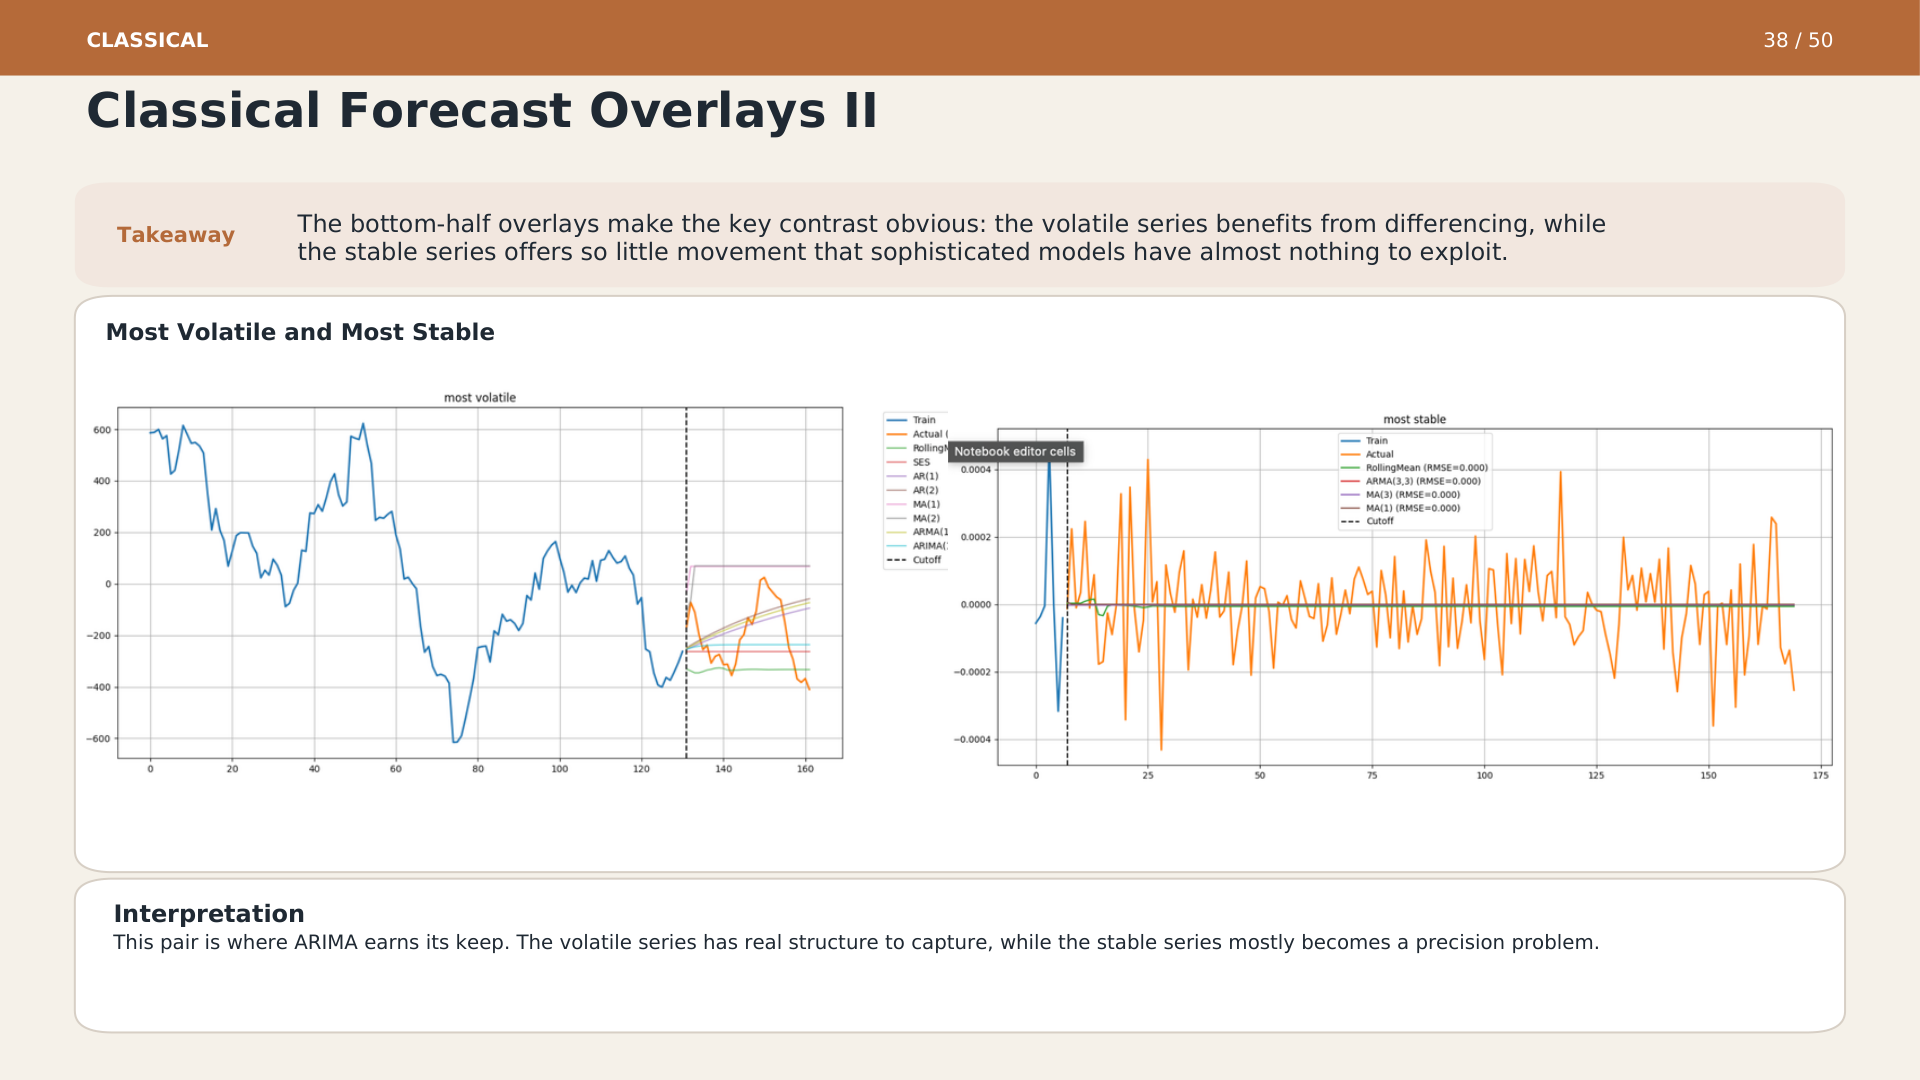
\includegraphics[width=0.95\textwidth]{figures/slide_34.png}
\caption{Classical forecast overlays for the most volatile and most stable representative series. The volatile series benefits from differencing---AR(1) captures short-lag persistence---while the stable series offers so little movement that sophisticated models have almost nothing to exploit.}
\label{fig:classical_forecasts}
\end{figure}

\begin{figure}[H]
\centering
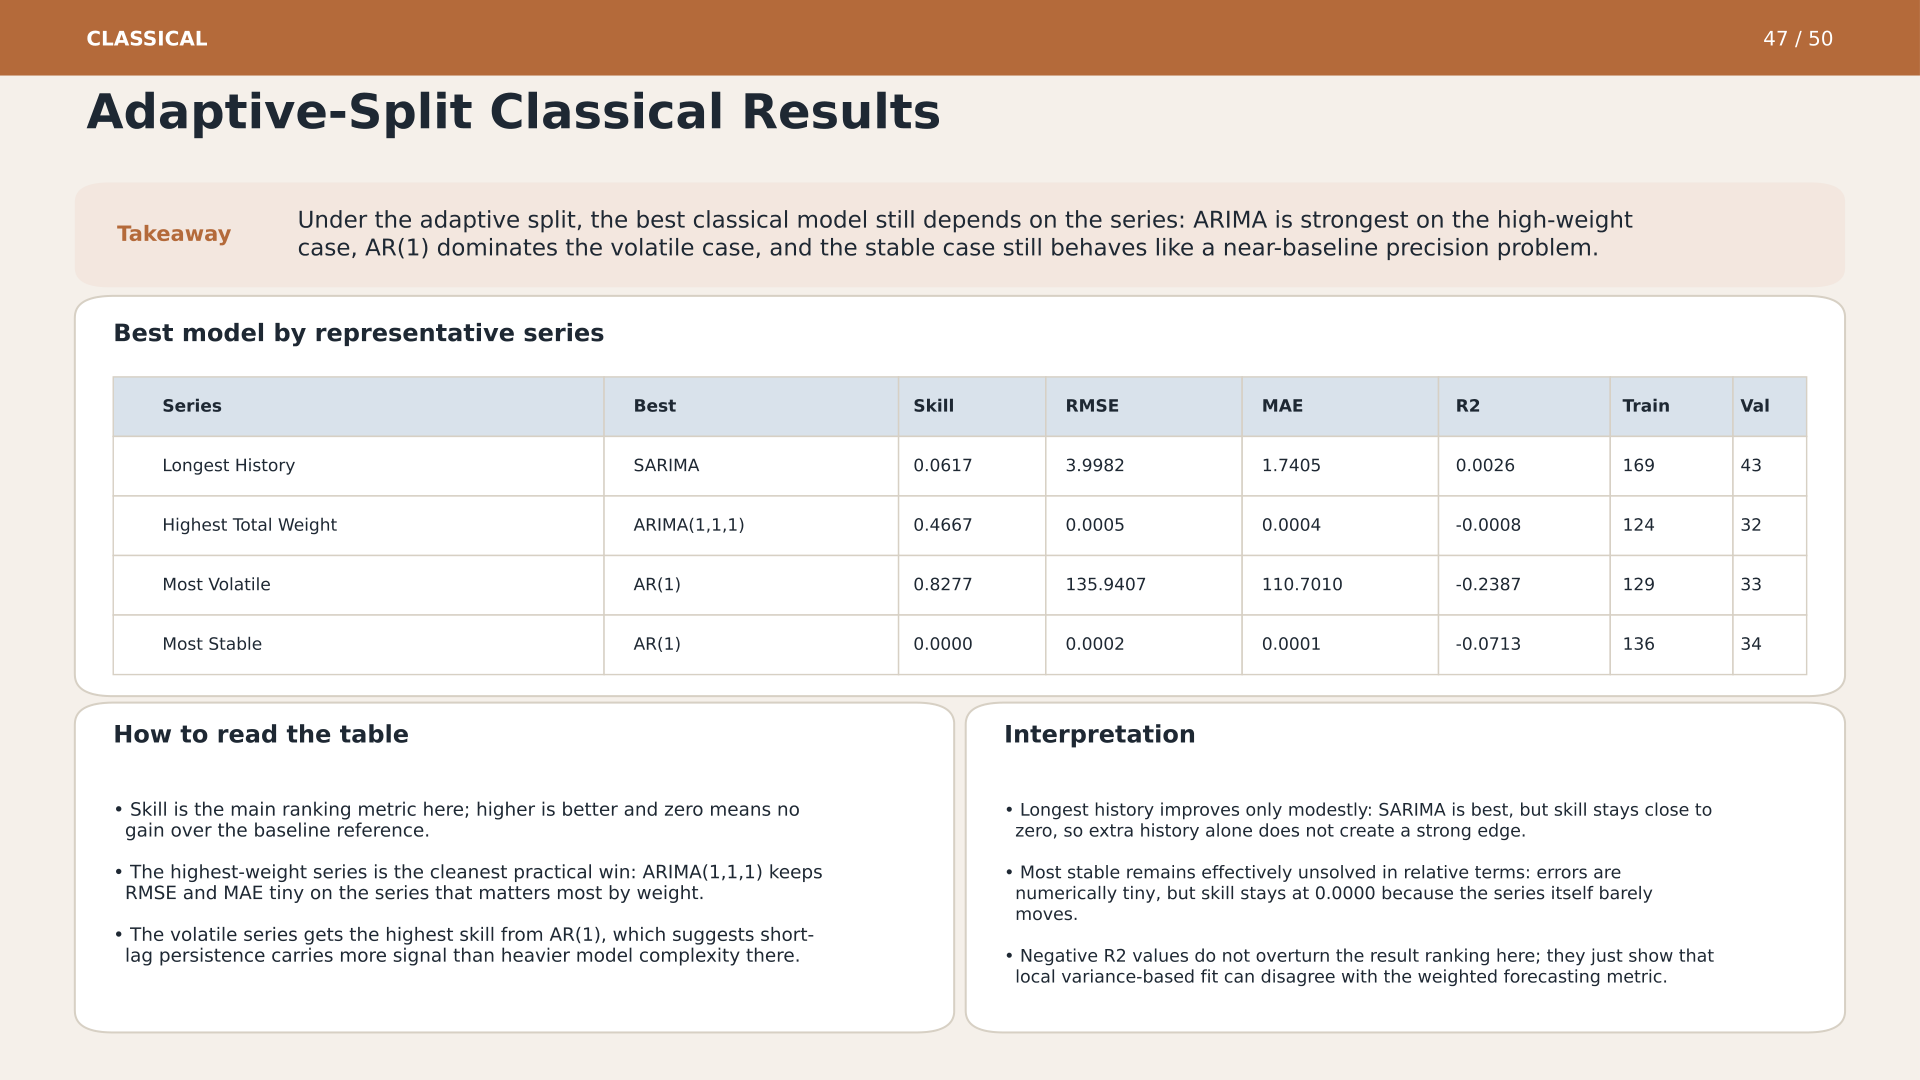
\includegraphics[width=0.95\textwidth]{figures/slide_38.png}
\caption{Adaptive-split classical results. Per-series best models: SARIMA wins on the longest-history series (skill 0.06), ARIMA(1,1,1) is strongest on the high-weight case (skill 0.47), AR(1) dominates both the volatile (skill 0.83) and stable (skill 0.00) cases. The volatile series has the most exploitable structure.}
\label{fig:classical_results}
\end{figure}

\subsubsection{The Stationarity Validation}

The $d=0$ versus $d=1$ comparison provides empirical validation of the EDA's stationarity finding:

\begin{itemize}
    \item Across matched-order pairs (e.g., ARIMA(1,0,0) vs. AR(1) $\equiv$ ARIMA(1,1,0)), the $d=1$ variant wins on the majority of series.
    \item This confirms that first differencing is genuinely beneficial for this dataset, not just a theoretical assumption.
\end{itemize}

\subsection{Deep Learning Performance Summary}

The three recurrent architectures generally show:

\begin{itemize}
    \item \textbf{LSTM and GRU} tend to outperform vanilla RNN, consistent with their superior gradient flow properties.
    \item Performance varies considerably across series, with some series showing substantial improvement over classical baselines and others showing degradation.
    \item Error accumulation in recursive forecasting is a significant factor, particularly for longer validation horizons.
\end{itemize}

\begin{figure}[H]
\centering
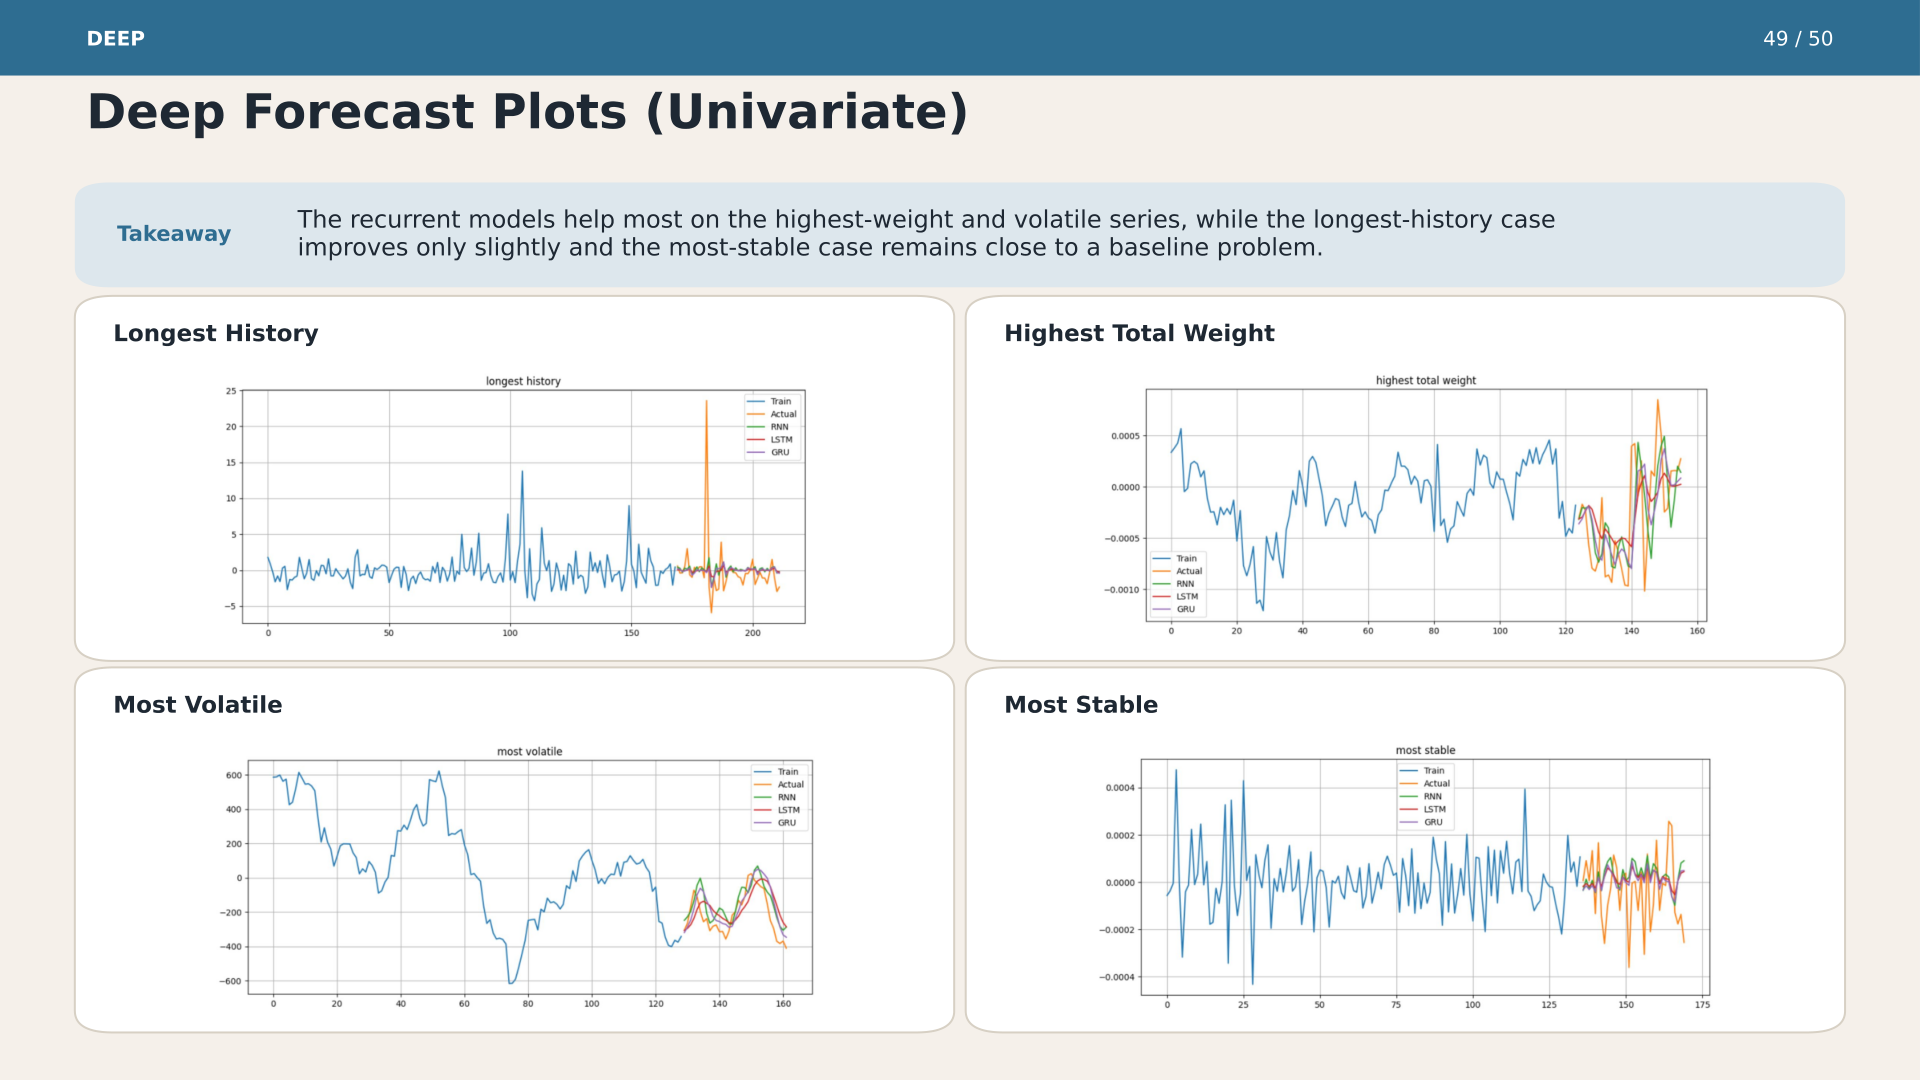
\includegraphics[width=0.95\textwidth]{figures/slide_40.png}
\caption{Deep forecast plots (univariate) for four representative series. The recurrent models help most on the highest-weight and volatile series, while the longest-history case improves only slightly and the most-stable case remains close to a baseline problem. Each panel shows Train (blue), Actual validation (orange), and overlaid RNN/LSTM/GRU predictions.}
\label{fig:deep_forecasts}
\end{figure}

\begin{figure}[H]
\centering
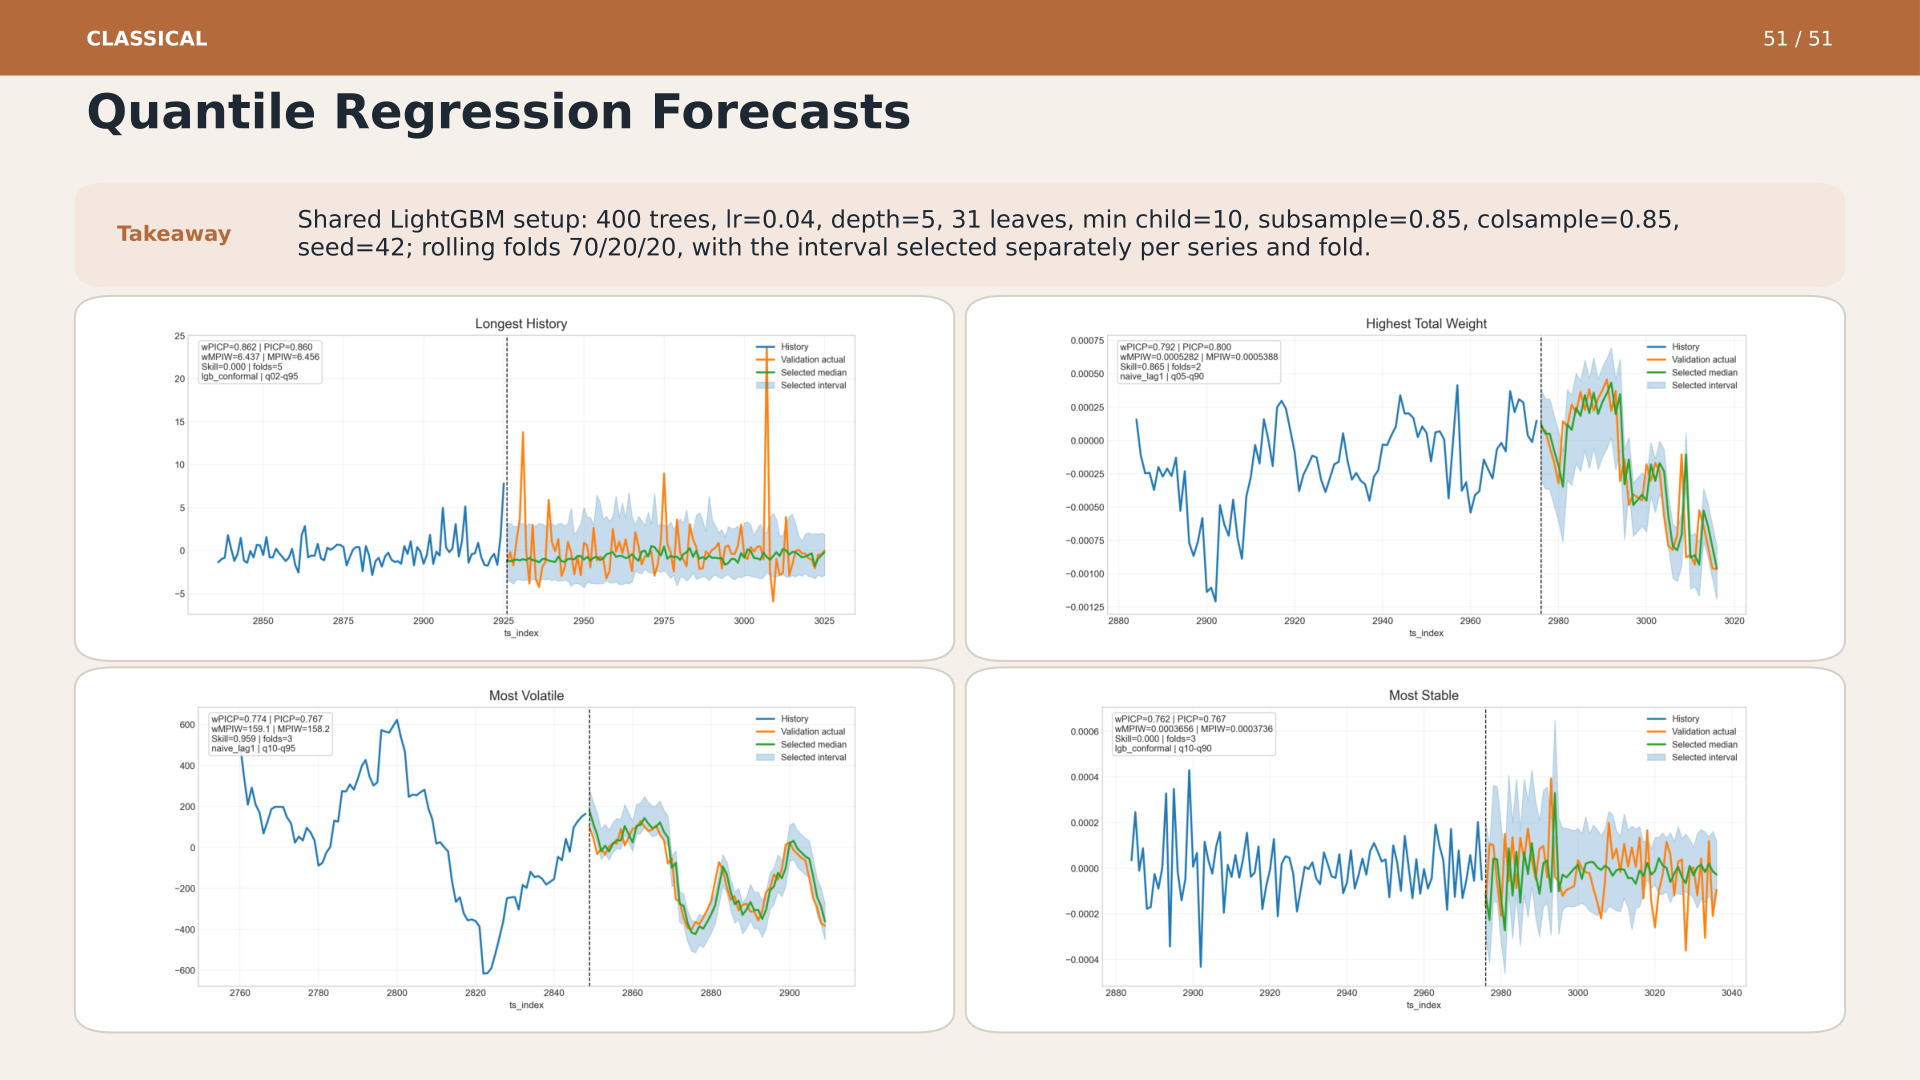
\includegraphics[width=0.95\textwidth]{figures/slide_42.png}
\caption{Quantile regression forecasts using LightGBM. Each panel shows the training history (blue), validation actuals (orange), selected median forecast (green), and prediction intervals (shaded blue). The model achieves PICP values between 0.76--0.86 across the four representative series.}
\label{fig:quantile_regression}
\end{figure}
To quantify uncertainty, quantile regression was implemented using LightGBM. Instead of point forecasts, the model predicts the conditional quantiles (e.g., 10th, 50th, and 90th percentiles), providing prediction intervals that capture the heteroskedasticity of financial returns.

